\newpage
\section{実験機材の説明}
\subsection{観測系の装置}
\subsection*{亜酸化銅結晶試料}
今回の実験で用いたのはナミビア産の天然亜酸化銅結晶である。
人工的に作り出すことはできるが、不純物や高純度性の観点から天然結晶を用いている。
結晶は大きさは5.3\,\text{mm} \times 5.3\,\text{mm} \times 8.0\,\text{mm}の寸法の直方体である。

\subsection*{希釈冷凍機}
\begin{figure}[htbp]
\begin{center}
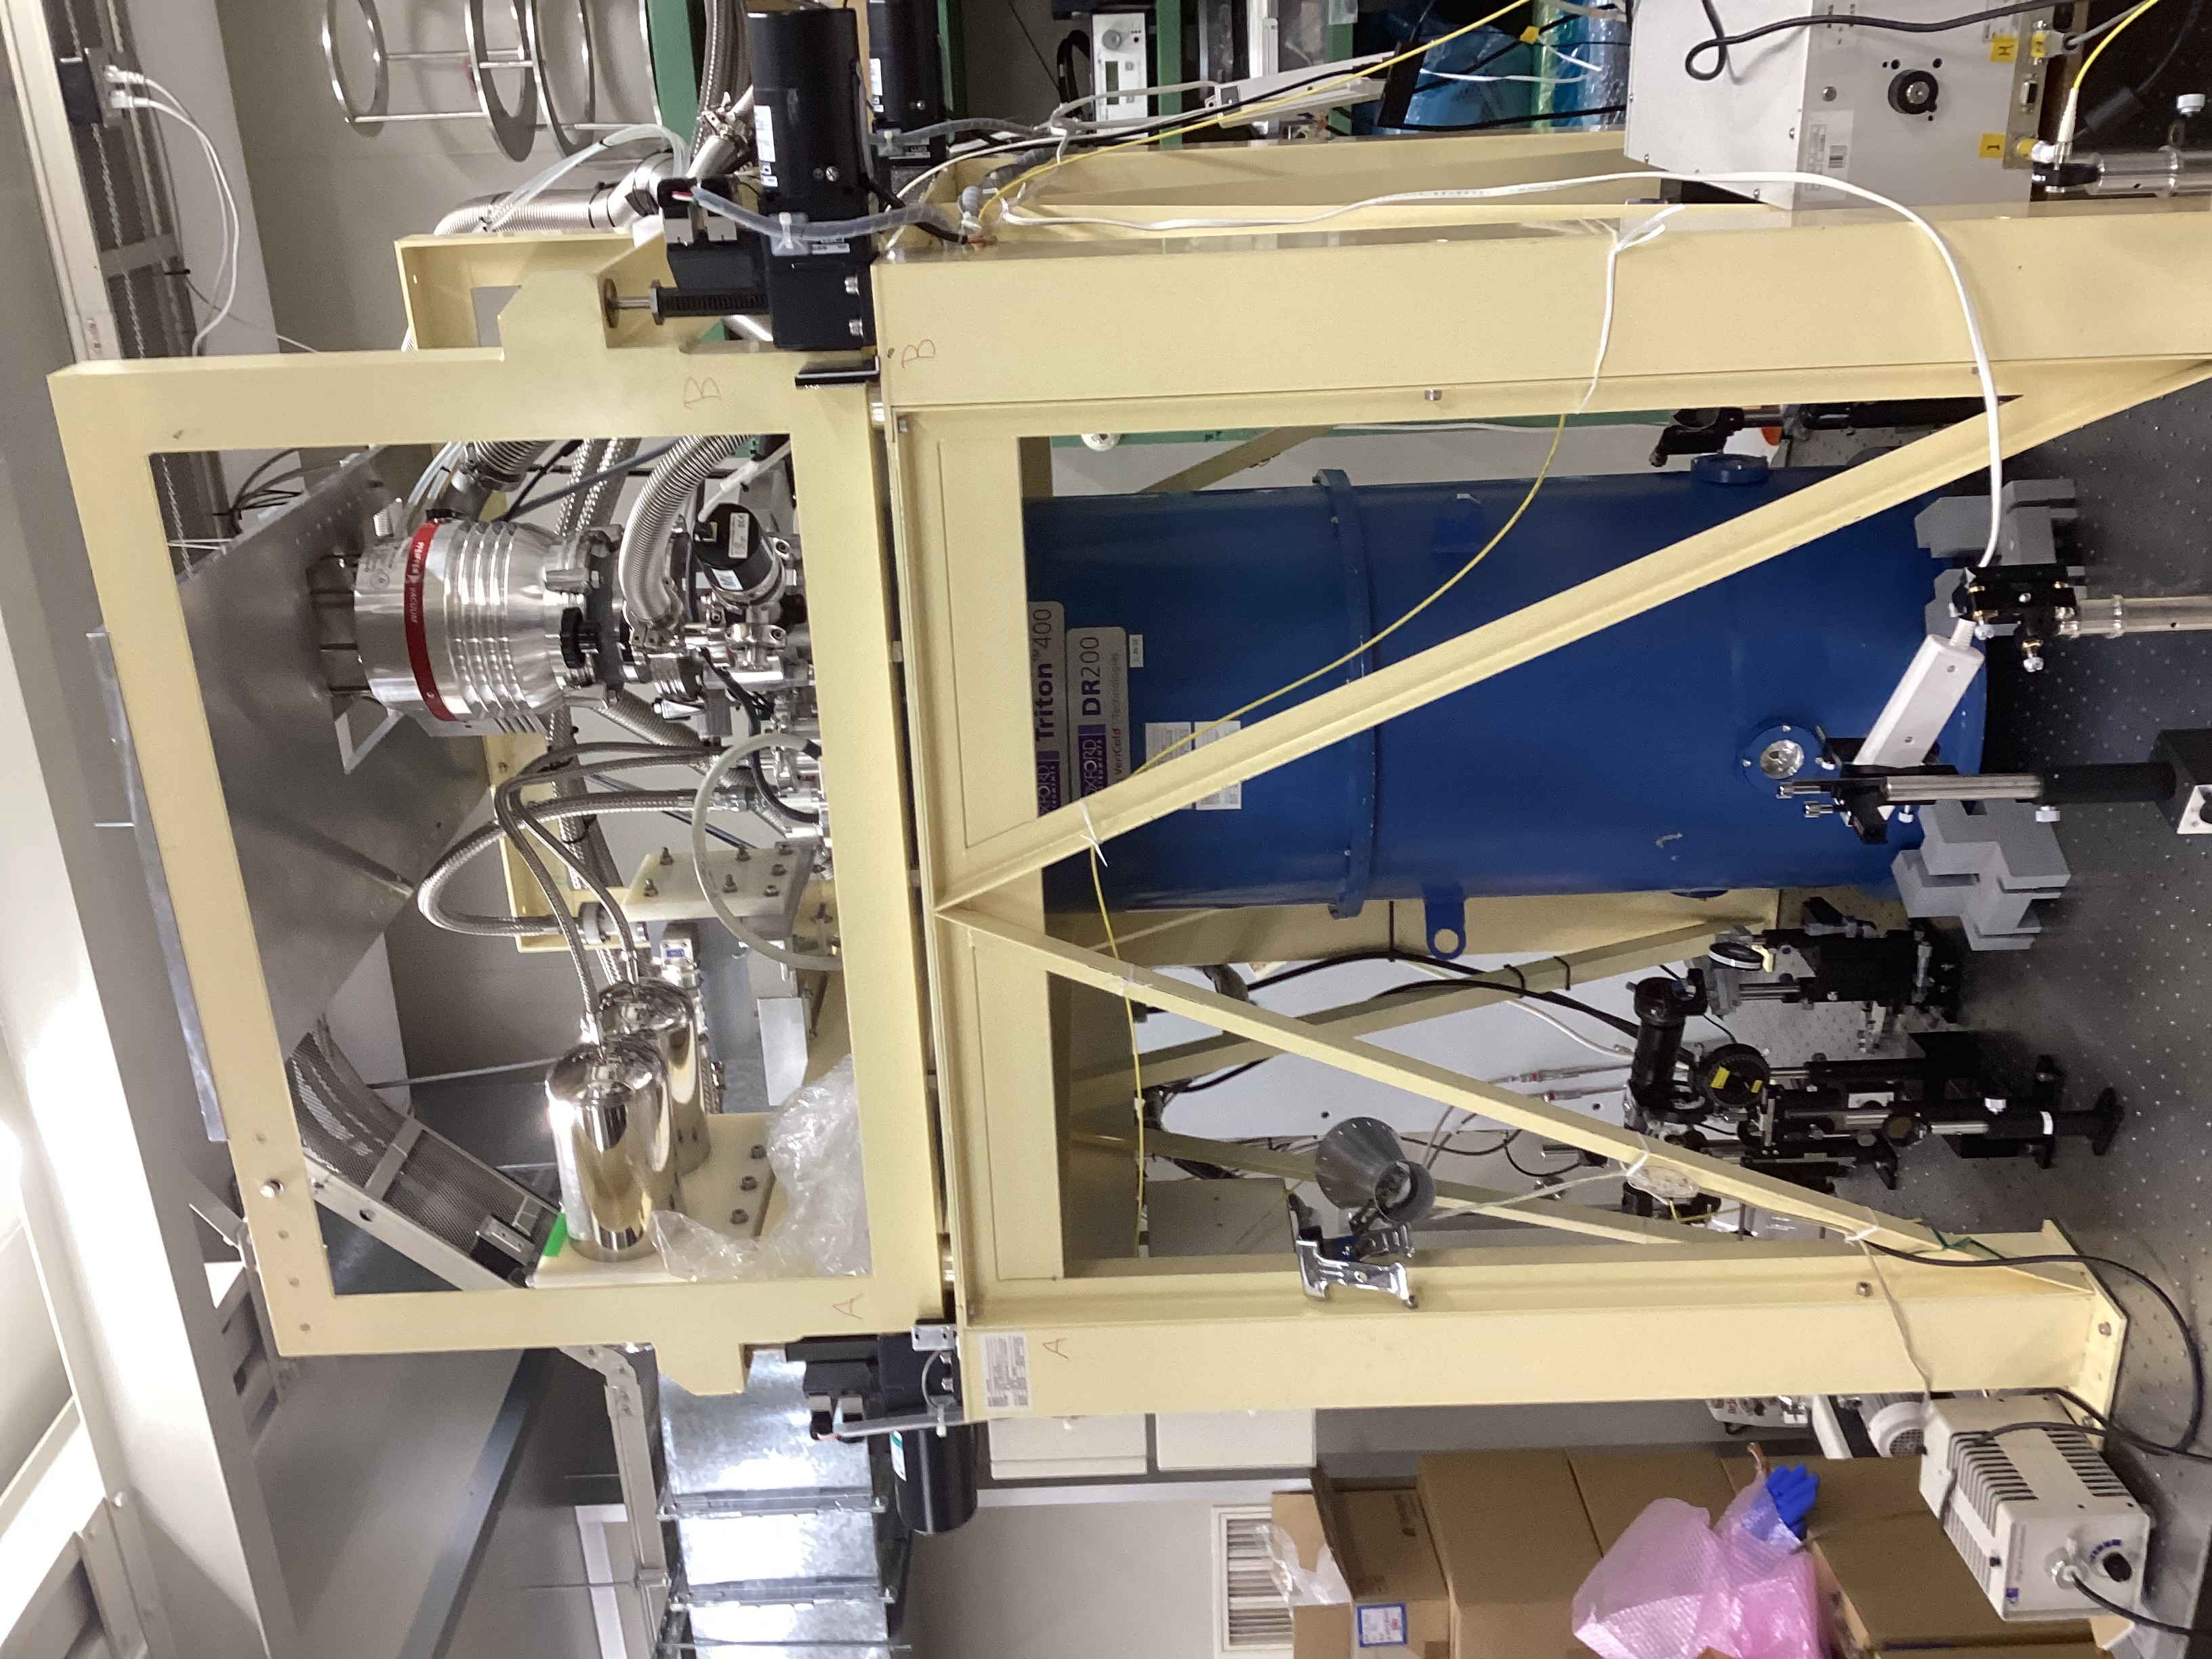
\includegraphics[width=100mm, angle=270]{IMG_8626.jpeg}
\caption{無冷媒希釈冷凍機}
\end{center}
\end{figure}
結晶の冷却にはOxford Instruments社の無冷媒希釈冷凍機(DR-400)を用いている。
希釈冷凍機とは$^3$Heと$^4$Heの混合液の相分離におけるエントロピー差を利用した冷却に実現している。
この冷凍機では、長期間にわたり低温環境を安定的に維持することが可能であり、設計上無冷媒であることからメンテナンスフリーであり数ヶ月にわたる運転が可能である。
理論上では、無限に低い温度環境を維持することが可能であるが、実際には外部からの熱流入が最低温度の限界を決定する。
電気抵抗に電流を流すことで熱を発生させ、冷却対象の温度を制御することができる。
DR-400には、励起光やプローブ光を入射するために窓が付けられている。
窓の設計は低温環境を維持するために様々な工夫がなされている。
温度はどこまでを維持れるんだっけ?希釈冷凍機では数十mKまでを達成することができるが、今回の実験のセットアップでは最低温度64 mKが達成可能である。
運転中に混入する不純ガスは、希釈冷凍機の性能を低下させる原因となる。
これを防ぐために外部でLN2 trapを使用することで不純ガスを回収する。
希釈冷凍機のサンプルステージには、不均一な応力印加用のレンズ(圧力印加用レンズ)と微弱な励起子の集光用のレンズ(発光観測用のレンズ)が設置されている。
それぞれ電圧を印加することで精密な位置操作を実現するピエゾを用いている。

\subsection*{複屈折の観測}
ピエゾ素子に電圧をかけること
材料が異方性を持つために、光が二つの異なる経路に分かれて進む現象のことである。
それぞれ二つの波がそれぞれ異なる屈折率をもつ。
ニコル配置
この実験ではピエゾ素子をねじまきがついている回転盤につけることによって上下の運動を制御することができる。
という値をもつ。

\subsection{エネルギーシフトの計算方法}
\begin{align}
    u(y, z, r_0) &= \frac{1}{2} \left( y^2 + z^2 - r_0^2 + \sqrt{(y^2 + z^2 - r_0^2)^2 + 4 r_0^2 z^2} \right) \\
    \sigma_{xx}(y, z, r_0, p_0, \nu) &= -p_0 \left[
        \begin{cases} 
            0 & (y = 0) \\
            \frac{(1 - 2\nu) r_0^2}{3 (y^2 + \epsilon)} \left( 1 - \left( \frac{z}{\sqrt{U}} \right)^3 \right) & (y \neq 0)
        \end{cases}
        + \frac{z}{\sqrt{U}} \left( 2\nu + \frac{(1 - \nu) U}{r_0^2 + U + \epsilon} - \frac{(1 + \nu) \sqrt{U}}{r_0} \arctan \left( \frac{r_0}{\sqrt{U}} \right) \right)
    \right] \\
    \sigma_{yy}(y, z, r_0, p_0, \nu) &= -\sigma_{xx} - \sigma_{zz} + 2 p_0 (1 + \nu) \frac{z}{\sqrt{U}} \left(
        -1 + \frac{\sqrt{U}}{r_0} \arctan \left( \frac{r_0}{\sqrt{U}} \right)
    \right) \\
    \sigma_{zz}(y, z, r_0, p_0) &= -p_0 \frac{\left( \frac{z}{\sqrt{U}} \right)^3 r_0^2 U}{U^2 + r_0^2 z^2} \\
    \sigma_{yz}(y, z, r_0, p_0) &= -p_0 \frac{y z^2 r_0^2 \sqrt{U}}{(U^2 + r_0^2 z^2)(r_0^2 + U)} \\
    \sigma_{xy}(y, z, r_0, p_0) &= 0 \\
    \sigma_{zx}(y, z, r_0, p_0) &= 0
\end{align}

$p_0$ は接触部分にかかる圧力を表し、
\begin{equation}
p_0 = \frac{3 F_0}{2 \pi r_0^2}
\end{equation}

という値を持つ。他の値については

\begin{equation}
\left\{
\begin{aligned}
F_0 &: \text{加える力} \\
R &: \text{結晶を押す物質の曲率半径} \\
E &: \text{結晶のヤング率} \\
\nu &: \text{結晶のポアソン比} \\
E_{\text{push}} &: \text{結晶を押す物質のヤング率} \\
\nu_{\text{push}} &: \text{結晶を押す物質のポアソン比}
\end{aligned}
\right.
\end{equation}

\begin{align*}
F_0 &= 160~\text{N} && \text{外力} \\
R &= 15.57 \times 10^{-3}~\text{m} && \text{曲率半径} \\
E &= 237 \times 10^{8}~\text{Pa} && \text{結晶のヤング率} \\
\nu &= 0.445 && \text{結晶のポアソン比} \\
E_{\text{push}} &= 801 \times 10^{8}~\text{Pa} && \text{結晶を押す材料のヤング率} \\
nu_{\text{push}} &= 0.208 && \text{結晶を押す材料のポアソン比}
\end{align*}

加える力 \( F_0 \) は外力の大きさとして \( 160~\text{N} \) であり、結晶を押す物質の曲率半径 \( R \) は \( 15.57 \times 10^{-3}~\text{m} \) です。また、結晶のヤング率(Young's modulus) \( E \) は \( 237 \times 10^{8}~\text{Pa} \)、ポアソン比(Poisson's ratio) \( \nu \) は \( 0.445 \) です。さらに、結晶を押す物質のヤング率 \( E_{\text{push}} \) は \( 801 \times 10^{8}~\text{Pa} \)、ポアソン比 \( \nu_{\text{push}} \) は \( 0.208 \) となっています。


応力テンソルから歪テンソルからの変換は弾性コンプライアンス定数を通して関連づけられる。
\begin{equation}
\begin{pmatrix}
    \epsilon_{xx} \\
    \epsilon_{yy} \\
    \epsilon_{zz} \\
    \epsilon_{xy} \\
    \epsilon_{yz} \\
    \epsilon_{zx}
\end{pmatrix} = 
\begin{pmatrix}
    S_{11} & S_{12} & S_{12} & 0 & 0 & 0 \\
    S_{12} & S_{11} & S_{12} & 0 & 0 & 0 \\
    S_{12} & S_{12} & S_{11} & 0 & 0 & 0 \\
    0 & 0 & 0 & \frac{S_{44}}{2} & 0 & 0 \\
    0 & 0 & 0 & 0 & \frac{S_{44}}{2} & 0 \\
    0 & 0 & 0 & 0 & 0 & \frac{S_{44}}{2}
\end{pmatrix}
\begin{pmatrix}
    \sigma_{xx} \\
    \sigma_{yy} \\
    \sigma_{zz} \\
    \sigma_{yz} \\
    \sigma_{zx} \\
    \sigma_{xy}
\end{pmatrix}
\end{equation}

以下に歪み(Strain)計算に使用する材料定数を示します。
結晶の弾性コンプライアンス定数として、\( S_{11} = 4.17 \times 10^{-11}~\text{Pa}^{-1} \)、\( S_{12} = -1.94 \times 10^{-11}~\text{Pa}^{-1} \)、および \( S_{44} = 8.26 \times 10^{-11}~\text{Pa}^{-1} \) が得られています。

材料に歪みが加わることでハミルトニアンが変化します。歪みの大きさが小さい場合、この変化を摂動として扱うことが可能です。摂動ハミルトニアン $H_{\text{deformation}}$ は、歪テンソルおよびデフォーメーションポテンシャルの定数によって表現されます。
\begin{align}
H_{\text{deformation}} &= a \, \operatorname{Tr}\, \epsilon 
- 3b \left[ \left(L_z^2 - \frac{1}{3} L^2 \right)\epsilon_{zz} 
+ \left(L_y^2 - \frac{1}{3} L^2 \right)\epsilon_{yy} 
+ \left(L_x^2 - \frac{1}{3} L^2 \right)\epsilon_{xx} \right] \\
&\quad - \sqrt{3}\,d \left[ (L_z L_y + L_y L_z)\epsilon_{xy} 
+ (L_y L_x + L_x L_y)\epsilon_{yx} 
+ (L_z L_x + L_x L_z)\epsilon_{zx} \right]
\end{align}

ここで、$a$ は等方的なデフォーメーションポテンシャル、$b$ と $d$ はそれぞれ剪断変形に関連するポテンシャル、$L$ およびその成分 $L_x$, $L_y$, $L_z$ は角運動量演算子を示します。
この摂動ハミルトニアンに対して、オルソ励起子およびパラ励起子に対する二次の摂動まで考慮することで、歪みによるエネルギーの変動を精密に評価できます。
三重に縮退したオルソ励起子に対する一次摂動ハミルトニアンは以下のように記述されます。固有関数を解析することで、縮退が解消されたオルソ励起子のエネルギー準位を導出できます。(ここで、$\eta = \frac{4|a|}{E_{\text{so}}}$ と定義します)

\begin{equation}
H_1^{\text{ortho}} = a \, \text{Tr}\,e \begin{pmatrix}
1 & 0 & 0 \\
0 & 1 & 0 \\
0 & 0 & 1 \\
\end{pmatrix} + \eta \begin{pmatrix}
b(2e_{xx} - e_{yy} - e_{zz}) & \sqrt{3d}\,e_{xy} & \sqrt{3d}\,e_{zx} \\
\sqrt{3d}\,e_{xy} & b(2e_{yy} - e_{xx} - e_{zz}) & \sqrt{3d}\,e_{yz} \\
\sqrt{3d}\,e_{zx} & \sqrt{3d}\,e_{yz} & b(2e_{zz} - e_{xx} - e_{yy}) \\
\end{pmatrix}
\end{equation}

一方、パラ励起子に対する一次摂動によるエネルギー変化は以下のように表されます。
\begin{equation}
\Delta E_1^{\text{para}} = a \, \text{Tr}\,e
\end{equation}

さらに、二次摂動によるエネルギー変動 $\Delta E_2$ を計算すると、オルソ励起子およびパラ励起子の両方に対して同一の値が得られます。これは価電子帯のエネルギーが上昇するため、励起子のエネルギーは負方向にシフトします。
\begin{equation}
\Delta E_2 = \frac{(3b)^2}{E_{\text{so}}} \left\{(e_{xx} - e_{yy})^2 + (e_{yy} - e_{zz})^2 + (e_{zz} - e_{xx})^2 \right\} + \frac{2(3d)^2}{E_{\text{so}}} \left(e_{xy}^2 + e_{yz}^2 + e_{zx}^2\right)
\end{equation}

デフォーメーションポテンシャルの具体的な値は以下の通りとします。
結晶のエネルギーパラメータとして、\( a = -1.18 \, \text{eV} \)、\( b = -0.40 \, \text{eV} \)、および \( d = 0.31 \, \text{eV} \) です。また、交換相互作用定数は \( J = 23.8 \, \text{eV} \)、スピン軌道結合エネルギーは \( E_{\text{so}} = 131 \, \text{meV} \) です。さらに、無次元パラメータ \( \eta \) は \( \eta = \frac{4|a|}{E_{\text{so}}} = 0.727 \) となります。


これらの式を計算することで1s励起子(パラ/オルソ)のエネルギー変移 $\Delta E_1^{\text{para/ortho}} - \Delta E_2$ を求めることができる。

Trauernichit1986によると[100]方向



\subsection{励起光の実験装置}
\subsubsection*{再生増幅機}
励起子の生成するための励起光の発生源として再生増幅機(Coherent INc 社製 Libra HE)を使用している。
中心波長が800nmであり、パルス幅100 fsの高強度のパルス光を生成し、繰り返し周波数は1 kHzである。
再生増幅器はシード光(Vitesse)が初期の光パルスを提供し、キャビティ内で増幅媒体を何度も通過することでパルスが増幅される。十分に増幅された段階でパルスをキャビティ外に取り出す。
ポンプレーザー(Evolution-15)がシードレーザーを増幅する、最後にストレッチャー/コンプレッサーがパルス広がりを調整した後、強力なパルスに圧縮する。

\subsubsection*{光パラメトリック増幅器(OPA)}
再生増幅機で生成された光の中心波長を調整するためにOPA(Optical Parametric Amplifer: Light Conversion社 TOPAS)を用いた。
OPAでは入力されたシグナル光が非線形結晶を通過する際、ポンプ光との相互作用によシグナル光が増幅され、それと同時にアイドル光が生成される。
アイドル光は、信号光とエネルギーを共有する形で増幅を助ける役割を果たす。

\subsubsection*{CCDカメラ}
CCDカメラは光子を電荷に変換し、その電荷を転送して最終的にデジタル信号として読み出す半導体素子である。

\subsubsection*{分光器}
Spectra Pro-500iモデルを用いた。
回折格子、プリズム
コリメータ: 入射光を平行光にするためのレンズまたはミラー。
スペクトルの波長校正に関してはネオン輝線を用いた。
観測された3つのスペクトルに
参考値としては$609.616\mathrm{nm}$、$614.306\mathrm{nm}$、$609.616\mathrm{nm}$、$616.359\mathrm{nm}$のネオンの輝線を用いた。

\subsubsection*{EMCCDカメラ}
EMCCDカメラは電子増幅技術(Electron Multiplication)を利用して微弱な光信号を高感度で検出するカメラである。
各電子が他の電子を励起して数十倍から千倍に増幅される。
EMCCDカメラには1ピクセルあたり$16 \, \mu \text{m} \times 16 \, \mu \text{m}$の大きさのCCD素子が1600$\times$200で並んでいる。
200ピクセルは分光器に集光された光の縦方向の情報に対応する。

\subsubsection*{ICCDカメラ}

ICCDカメラはフォトカソードとMCPがある。高速現象観測、パルスレーザー測定に
微弱な励起光を検出するためにICCDカメラ(Andor社製 iStar)を用いた。
このICCDカメラでは1ピクセルあたり$13 \, \mu \text{m} \times 13 \, \mu \text{m}$の大きさのCCDが$1024 \times 1024$並んでいる。
externalモードをかけることでゲートをかけるタイミングは外部信号の立ち上がりまたは立ち下がりを時間原点として同期させることができる。

\subsection{全体の実験装置の概略}
実験装置のがいきこ

\subsection{エネルギーシフトの計算方法}
